%!TEX root = ../thesis.tex
%*******************************************************************************
%****************************** Second Chapter *********************************
%*******************************************************************************

\chapter{Marco teórico}

\ifpdf
    \graphicspath{{Chapter2/Figs/}{Chapter2/Figs/PDF/}{Chapter2/Figs/}}
\else
    \graphicspath{{Chapter2/Figs/}{Chapter2/Figs/}}
\fi


\section{Blockchain}
Blockchain o cadena de bloques es un registro público de transacciones que se
mantiene mediante una red distribuida de computadores, que no requiere respaldo de
ninguna autoridad central o una tercera parte y que ofrece un esquema transaccional
libre de intermediarios, gracias al uso de algoritmos criptográficos. Puede compararse con el libro
de registros de contabilidad de una empresa en donde se registran todas las entradas
y salidas de dinero, aunque en este caso hablamos de un libro de acontecimientos
digitales que no requiere de un intermediario centralizado que identifique y certifique la
información, sino que está distribuida en múltiples nodos independientes entre sí que
la registran y la validan sin necesidad de que haya confianza entre ellos.

Esta cadena de bloques (blockchain) consta de tres componentes fundamentales: transacciones,
registro y un sistema que las verifica y almacena en bloques. Cada bloque se genera a través de un
software que registra cronológicamente la información sobre cuándo y en qué secuencia han tenido
lugar las transacciones, de allí deriva su nombre. 
Esta tecnología permite que se realicen las transferencias electrónicas de una manera segura sin la
presencia de un tercero de confianza, dando solución a la principal barrera técnica de las últimas
décadas para los desarrolladores tecnológicos, el problema del doble gasto.

Por fuera de Blockchain, las transferencias electrónicas requieren intermediarios financieros para
dar confianza y seguridad a la transacción. Los intermediarios financieros generan confianza y
seguridad, preservando un registro único y centralizado de las operaciones electrónicas que permite
controlar los saldos de los titulares de cuentas y, en última instancia, garantizar la autenticidad
de una transacción. Sin intermediarios, las unidades de valor electrónicas -pesos o dólares- pueden
ser copiados y usados dos veces, tal como cualquier documento digital puede ser copiado
indefinidamente. En Blockchain, una vez introducida la información, no puede ser borrada o
modificada, solo se podrán añadir nuevos registros y no será legitimada a menos que la mayoría de
los actores se pongan de acuerdo para hacerlo.

Se podría entender esta tecnología con fundamento en sus tres características generales de la
siguiente forma: i) Blockchain es una tecnología "sin confianza", lo que significa que por primera
vez en la historia, intercambios de valor a través de una red de computadores pueden ser
verificados, monitoreados y asegurados sin la presencia de un tercero de confianza o
de una institución central; ii) es una tecnología de autenticación y verificación, que permite de
forma más eficiente las transferencias de títulos y la verificación de propiedad y iii) por ser una
tecnología sin fronteras y sin fricción, puede proporcionar una más económica y rápida
infraestructura para el intercambio de unidades de valor.

Esta tecnología surgió como el soporte tecnológico del Bitcoin y luego fue adoptada por múltiples
sectores en donde existía la necesidad de un registro o de intercambio de valor, como se verá más
adelante. Para comprender el funcionamiento general del Blockchain, se explicará la primera versión
que sirvió de base para los desarrollos en los que se está trabajando en la actualidad.


\subsection{¿Cómo funciona?}
Veremos más sobre el funcionamiento de Ethereum en otros capítulos. Aquí se intentará explicar de 
manera generalizada el funcionamiento de una blockchain.

Para generar un contexto, supondremos que Alpha quiere transferir a Beta una determinada
cantidad de unidades de valor (Alguna criptomoneda, pesos, dólares, etc.) y que ambos tienen acceso
a una billetera o un monedero en el celular, un computador o una web que les permite enviar o
recibir la moneda. Cuando Alpha decide gastar sus unidades de valor, lo que realmente está haciendo
es enviar una instrucción de cambio a la base de datos informando que parte de sus unidades de
valor ahora pertenecen a Beta. Esta instrucción es difundida en la red verificando que Alpha tiene
recursos para pagar y, si todo se encuentra correcto, se compila con otras transacciones
en un bloque con información relativa a los últimos diez minutos.
Este bloque mezcla la información de las direcciones de las partes involucradas en cada
transacción, la cantidad de unidades de valor en movimiento y una marca de tiempo, y luego las
procesa a través de una función llamada Hash. Esta función es un algoritmo criptográfico, que se
encarga de condensar en un único digito de 64 caracteres información de cualquier extensión.
Por ejemplo, el hash (encriptado con el algoritmo SHA-256) para la palabra “blockchain” sería
EF7797E13D3A75526946A3BCF00DAEC9FC9C9C4D51DDC7CC5DF888F74DD434D1 y el de “Blockchain”
625DA44E4EAF58D61CF048D168AA6F5E492DEA166D8BB54EC06
C30DE07DB57E1. Preste especial atención que ante cambios como la capitalización de una letra o la
longitud del texto, el hash es completamente diferente.

Este hash se combina con la solución-hash del bloque anterior, y se convierte en el encabezado del
bloque nuevo que se encuentra en validación. A su vez este es la base de un problema matemático que
se resuelve usando de nuevo la función Hash. La respuesta a este acertijo es solucionado por la red
en un proceso de prueba y error. Cuando finalmente algún nodo de la red encuentra la solución, esta
es compartida con el resto para su validación, en un proceso llamado “proof of work” (prueba de
trabajo). Después que ha sido aprobada por la mayoría de la red, el bloque es añadido a la cadena y 
con ello todas las transacciones contenidas en él, incluido el pago de Alpha hacia Beta.

La blockchain establece la confianza entre dos partes en una transacción a través de un libro de 
contabilidad público descentralizado y un mecanismo criptográfico que garantiza que las 
transacciones no pueden cambiarse después de materializadas.

\section{Ethereum}
Ethereum aparece a finales del año 2013 en un paper publicado por Vitalik Buterin con el objetivo
de proveer un sistema descentralizado capaz de correr aplicaciones casi sin límite de capacidades.

Ethereum es una red peer-to-peer (p2p) de máquinas virtuales que cualquier desarrollador puede
utilizar para ejecutar aplicaciones distribuidas (dApps). Estos programas informáticos pueden ser
cualquier cosa, pero la red está optimizada para llevar a cabo reglas que se ejecutan mecánicamente
cuando se cumplen ciertas condiciones, como un contrato. Ethereum utiliza su propia blockchain
pública descentralizada para almacenar, ejecutar y proteger criptográficamente estos contratos. 
Cada computadora de su red descarga una pequeña máquina virtual para sincronizarse con la
blockchain de Ethereum y volver a estar disponible para ejecutar contratos. Esta red distribuida de
computadoras proporciona convenientemente la seguridad, confiabilidad y potencia de computación
necesarias para llevar a cabo los arreglos diseñados. Por supuesto, esta red de consenso no es
gratuita ni privada, por lo que los desarrolladores sólo la utilizan para llegar a un consenso
sobre los resultados y cuando sus datos pueden ser públicos.

La intención de Ethereum es crear un protocolo alternativo para la construcción de dApps,
proporcionando un conjunto diferente de compensaciones que se cree serán muy útiles para una gran
clase de aplicaciones descentralizadas, con especial énfasis en situaciones en las que el tiempo de
desarrollo rápido, la seguridad para aplicaciones pequeñas y poco utilizadas, y la capacidad de las
 diferentes aplicaciones para interactuar muy eficientemente, son importantes.
 
\begin{wrapfigure}{l}{0.7\textwidth}
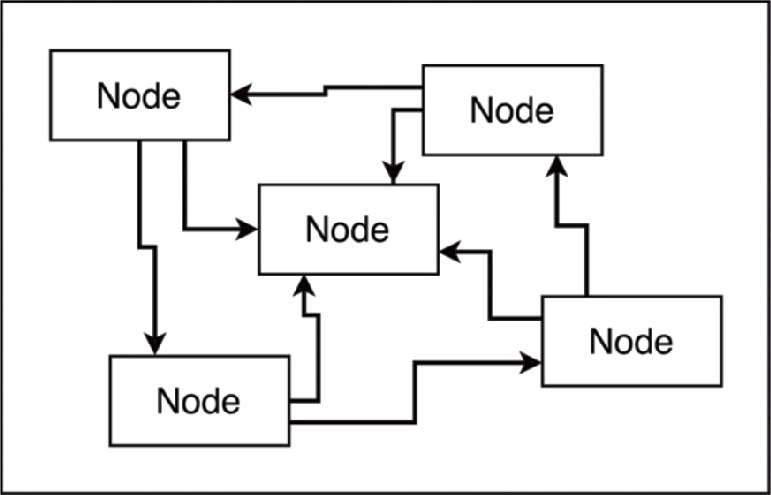
\includegraphics[width=0.7\linewidth]{ethereum-nodes} 
\caption[EthereumNodes]{Los Nodos de Ethereum se interconectan entre sí (P2P)}
\label{fig:ethereum-nodes}
\end{wrapfigure} 
 
Ethereum hace esto construyendo lo que es esencialmente la última capa fundacional abstracta: una
blockchain con un lenguaje de programación Turing completo integrado, que permite a cualquiera
escribir contratos inteligentes y aplicaciones descentralizadas donde puede crear sus propias
reglas arbitrarias para la propiedad, formatos de transacción y funciones de transición de estado.


\subsection{Fíat Currency (dinero fiduciario)}
Comúnmente se dice que el bitcoin no está respaldado por nada, y eso es cierto. Las monedas fiat
modernas tampoco están respaldadas por nada, sin embargo, son diferentes: endosados
por un gobierno, una moneda fiduciaria es mantenida por defecto por cualquiera que pague impuestos
y compre bonos del Estado. Algunas ventas internacionales de materias primas están denominadas en
dólares, también (por ejemplo, el petróleo) dando a la gente otra razón para retener dólares.

En el caso de las criptomonedas, persisten los problemas de adopción. Hoy en día, estos tokens
digitales siguen siendo una capa de pago público, rápido y seguro en la parte superior del sistema
de dinero fiduciario existente; un despliegue experimental que podría algún día crecer para
reemplazar los pagos centralizados utilizadas hoy en día por empresas como Visa y MasterCard.

Se vislumbran grandes posibilidades en el horizonte, ya que los gobiernos y el sector privado s
encuentran en una situación difícil. Los inversores institucionales empiezan a crear grandes
mercados para los productos y servicios financieros denominadas en criptomonedas. Los bancos
centrales pueden incluso adoptar esta tecnología. Al menos un país ha emitido un dólar digital
utilizando el software Bitcoin: Barbados. Otros están investigando activamente el prospecto.


\subsubsection{Ether}
Hoy en día, Bitcoin (denotado por el símbolo BTC) es utilizado por personas, gobiernos y empresas
para transferir valor y comprar productos o servicios. Cada vez que envían bitcoins, pagan una
pequeña cuota a la red, que está denominada en bitcoins. Ether, denotado por el símbolo ETH, se
puede utilizar de forma similar. Para entender el camino a seguir, se necesita saber algunas cosas.

Primero, el ether tiene otro uso: puede pagar para ejecutar programas en la red de Ethereum.
Estos programas pueden transferir el ether ahora, o en el futuro, o cuando se cumplan ciertas
condiciones (especificadas en los contratos).
Debido a su capacidad de pagar por la ejecución de transacciones en el futuro, el ether puede
también ser considerado un producto básico, como el combustible para que la red ejecute
aplicaciones y servicios. Por lo tanto, tiene una dimensión adicional de valor intrínseco sobre los
bitcoins; no es sólo una reserva de valor.

Hoy en día, el abrumador uso de las monedas fiduciarias podría sugerir que
las criptomonedas son "peor dinero", es decir, más propensas a la inutilidad a largo plazo.
Y sin embargo, los bitcoins y el ether son famosamente acaparados por los poseedores, e incluso
mantenidos en un fideicomiso por al menos una compañía hasta el momento de escribir esto:
Grayscale, una subsidiaria de Digital Currency Group es un buen ejemplo.
Mientras tanto, los bancos centrales de Occidente experimentan con tipos de interés cercanos a cero
y flexibilización cuantitativa, también conocida como impresión de dinero, en una situación cada
vez más peligrosa y desesperada por mantener la inflación y la deflación bajo control.

Con la recompensa de bitcoin reduciéndose a la mitad cada cuatro años, la política monetaria
mundial se ve afectada. En general la incertidumbre económica, y la disminución de la confianza en
las monedas fiduciarias, enormes sumas de dinero latente en criptomonedas "acaparadas" están siendo
arrastradas al mercado por los precios más altos del servicio de demanda genuina. Esto se refleja
en los precios cada vez mayores de la mayoría de los tokens criptográficos, por muy volátiles que
sean sus precios intradía. Este acto de equilibrio entre acaparadores, especuladores, y
"derrochadores" crea un mercado próspero y saludable para la criptomoneda, y sugiere que
los criptokens como una clase de activos ya están sirviendo a los propósitos del dinero, y mucho
más.

El siguiente cuadro cortesía de https://www.cryptocurrencychart.com/ nos muestra el precio del 
bitcoin y del ether a lo largo del año 2018. Una conclusión rápida que vemos es que el ether es
bastante más estable en precio que el bitcoin.

\begin{figure}[htbp!] 
\centering    
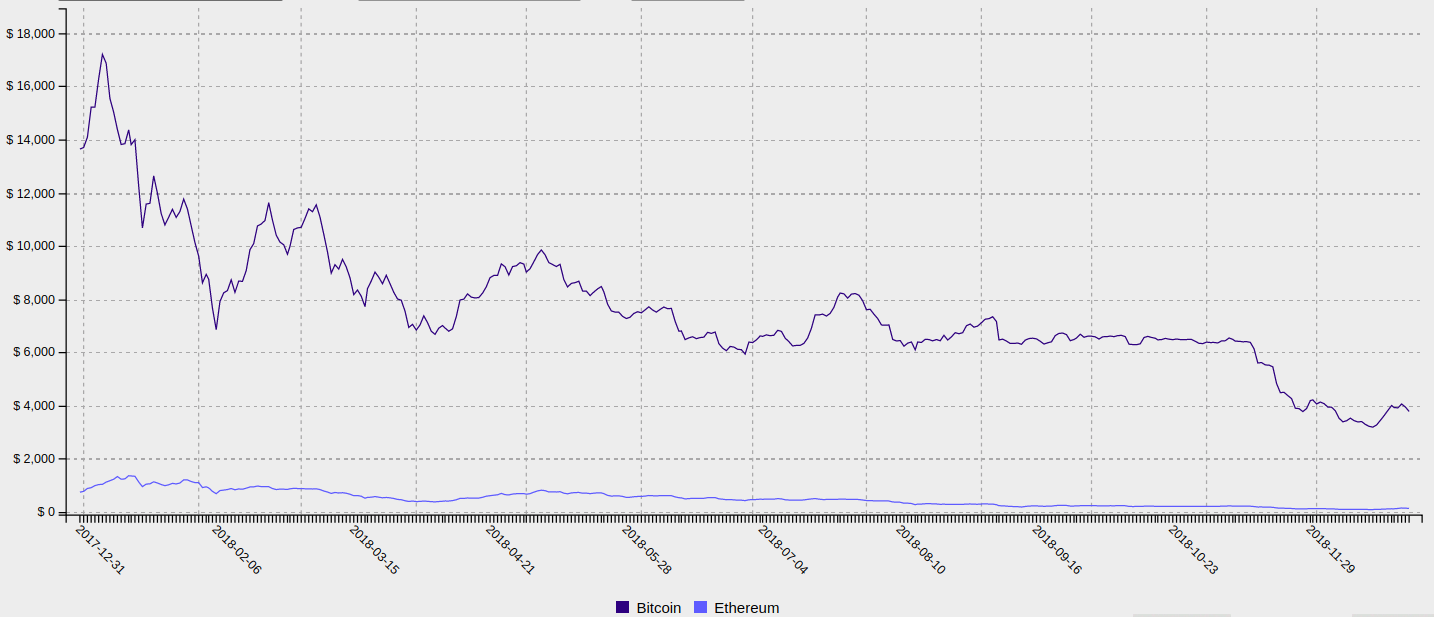
\includegraphics[width=0.9\textwidth]{ethbtc2018}
\caption[EthBtc2018]{Cuadro comparativo de precios entre Bitcoin y Ether durante 2018}
\label{fig:eth-btc-2018}
\end{figure}

\subsection{Protocolos}
Por definición, un protocolo en informática y telecomunicaciones es un sistema de normas que
regulan la comunicación entre dos o más sistemas que se transmiten información a través de 
diversos medios físicos.

Los protocolos pueden variar en gran manera, sin embargo, suelen tener al menos una de las 
siguientes propiedades:

\begin{itemize}
\item Detección de la conexión física subyacente.
\item Negociación de características de conexión.
\item Política de corrección de errores.
\item Establecimiento de la conexión y su término.
\item Qué hacer en caso de pérdida repentina de la conectividad.
\item Estrategias de seguridad o cifrado.
\item Formato de los mensajes.
\end{itemize}


\subsubsection{Ethereum Wire Protocol}
%@TODO

\subsection{Smart Contracts}
El término smart contract hace referencia a cualquier contrato que se ejecuta por sí mismo
automáticamente sin que medien terceros entre los participantes individuales. Los smart contracts
se escriben como programas informáticos en lugar de como lenguaje legal sobre documentos impresos.
El programa puede definir reglas y consecuencias estrictas del mismo modo que lo haría un documento
legal tradicional, pero a diferencia de los contratos tradicionales, también puede tomar
información como input, procesarla según las reglas establecidas en el contrato y adoptar cualquier
medida que se requiera como resultado de ello.

El concepto lo definió en 1994 el criptógrafo Nick Szabo, pero en la práctica no se hizo realidad
porque la infraestructura tecnológica necesaria para apoyarlo aún no existía. En la actualidad, con
la llegada de los protocolos de cifrado y el blockchain la situación cambió y, como resultado, la
idea ha vuelto a renacer.

En resumen, los contratos inteligentes son scripts modulares, repetibles y autónomos que
normalmente se ejecutan en una blockchain y representan promesas unilaterales de proporcionar una
tarea informática determinada. Estos scripts se almacenan en la blockchain, en una dirección
específica que se determina cuando se implementan los contratos en la blockchain. Cuando se produce
un evento contemplado en el contrato, se envía una transacción a esa dirección y la máquina virtual
distribuida ejecuta los códigos de operación del script (o cláusulas) utilizando los datos enviados
con la transacción.

Los contratos inteligentes pueden estar codificados de modo que reflejen cualquier tipo de lógica
empresarial basada en los datos: desde acciones tan sencillas como votar por una publicación en un
foro hasta acciones con un mayor nivel de complejidad, como garantías de préstamos y contratos de
futuros, así como acciones sumamente complejas como la fijación de prioridades de pago en una nota
estructurada.


\subsection{Solidity programming language}
Solidity es un lenguaje de programación de alto nivel "contract-oriented" usado para escribir
programas (smart contracts), que serán ejecutados por la EVM (Ethereum Virtual Machine). Su
sintaxis es muy similar a lenguajes como JavaScript o C.
Este lenguaje es una mezcla de convenciones de networking, lenguaje ensamblador, y desarrollo web.

Veremos más sobre él en capítulos posteriores.

\subsection{Base de datos distribuida, ¿Dónde están los datos?}
En Ethereum, la red es la base de datos. Todos los datos de los usuarios están almacenados en 
cada nodo de la red. Todas las transacciones en Ethereum se almacenan en la blockchain, un
historial cambios de estado es almacenados en cada nodo de Ethereum.

Cuando un usuario paga por el tiempo de computación en la red Ethereum, esto incluye el costo
de ejecutar la transacción y para el almacenamiento de los datos incluidos en su contrato
inteligente. (Si el contrato se hace más pequeño después de ejecutarse, el usuario recibirá un
reembolso parcial en forma de tarifa de transacción reducida.)

Tan pronto como se ejecute el smart contract y la tarifa en ether sea pagada, los datos serán
incluídos en el siguiente bloque. Debido a que la red Ethereum requiere que todos los nodos
mantengan el estado de todos los contratos, cualquier nodo puede consultar a la base de datos
local. Esto es sumamente poco escalable!



\section{Herramientas y tecnologías utilizadas}
\subsection{MetaMask}
MetaMask es una extensión del navegador, en este caso Google Chrome, la cual nos hace un puente
que permite conectarnos a las redes descentralizadas de Ethereum y visitar dApps en el navegador
sin necesariamente tener que montar un nodo Ethereum en nuestra máquina.

\begin{figure}[htbp!] 
\centering    
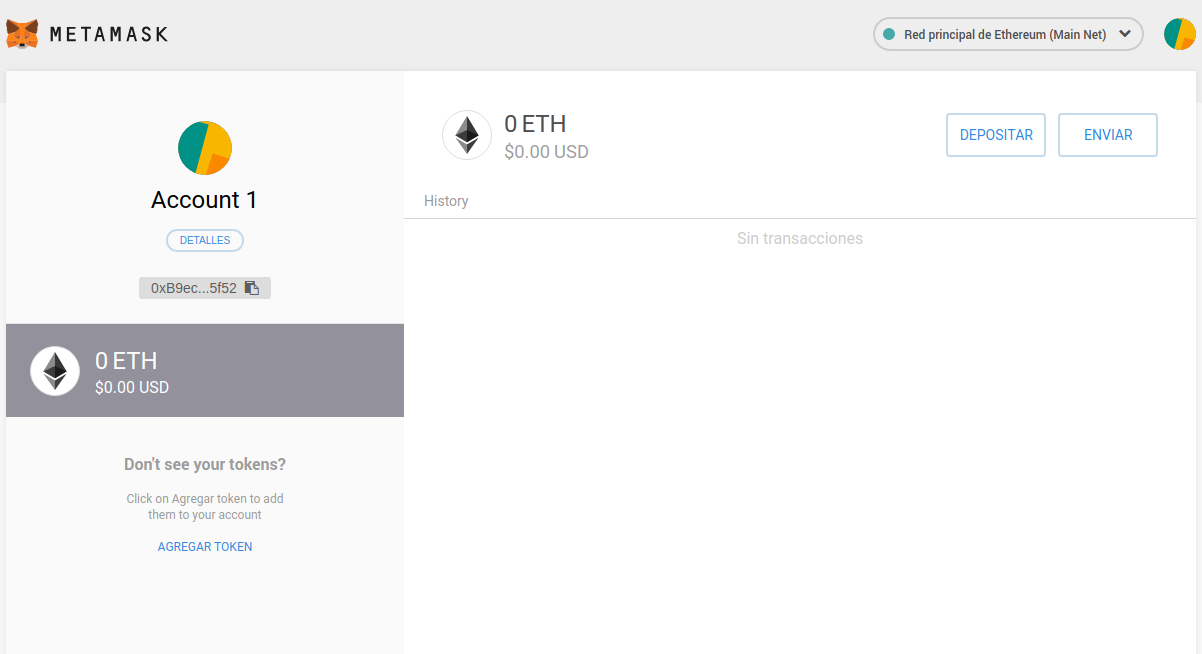
\includegraphics[width=0.7\textwidth]{metamask-main}
\caption[MetaMaskMain]{Así luce MetaMask recién instalado}
\label{fig:metamask-main}
\end{figure}

También en la siguiente figura podemos ver las opciones que nos ofrece MetaMask en cuanto 
a redes Ethereum para conectarnos. Tenemos un vasto catálogo, tanto redes de prueba, locales
como la red principal de Ethereum (lo que llamaríamos un entorno de producción).

\begin{figure}[htbp!] 
\centering    
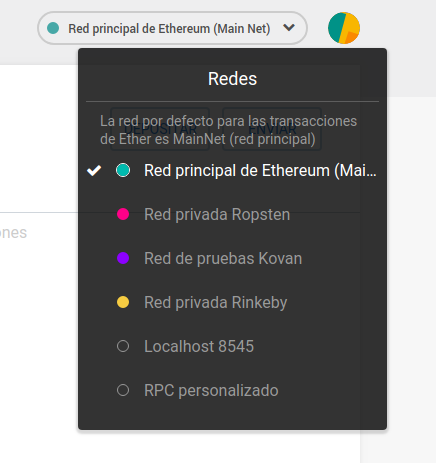
\includegraphics[width=0.8\textwidth]{metamask-networks}
\caption[MetaMaskNetworks]{Opciones de redes Ethereum que nos ofrece MetaMask}
\label{fig:metamask-networks}
\end{figure}

\subsection{Remix (remix.ethereum.org)}
Remix es una potente herramienta open source que nos permite escribir contratos en código
Solidity desde el browser, testearlos, deployarlos, debuggearlos, ver sus imputs y sus outputs
entre otras varias acciones. Es practicamente una IDE completa.

Está escrita en JavaScript y se encuentra en estado Alpha.

\subsection{JavaScript}
JavaScript es un lenguaje de programación interpretado, dinámico, de alto nivel y sin
tipos. Estandarizado por la especificación de lenguaje ECMAScript, fue diseñado originalmente para
ser utilizado del lado cliente y luego extendido para su uso del lado servidor. Es una de las tres
tecnologías fundamentales de la Web, junto con HTML y CSS. Su versión actual es ECMAScript 2018
(todavía no soportado "out of the box" por los navegadores).


\subsection{Node.js}
Node.js es un entorno de ejecución multiplataforma para el desarrollo de una variedad de
herramientas y aplicaciones del lado servidor construido con el motor de JavaScript V8 de Chrome.
Aunque no es un framework JavaScript, muchos de sus módulos básicos están escritos en JavaScript y
los desarrolladores pueden también escribir nuevos módulos con él. Tiene una arquitectura basada en
eventos y está enfocado en la optimización de escalabilidad y rendimiento para aplicaciones web que
utilicen un fuerte procesamiento asíncrono de entrada/salida. Desarrollado inicialmente por Ryan
Dahl en el año 2009 (Ryan ya no forma parte del proyecto), se encuentra actualmente en las
versiones 10.14.0 (LTS) y 11.5.0 (Current).

Para el presente trabajo utilizaremos la versión LTS (Long Term Support).


\subsubsection{Módulos utilizados}
En la siguiente sección se listarán y describirán los módulos de Node.js utilizados con el fin de
compilar, testear, deployar contratos y/o conectarse a una red Ethereum desde el entorno de
ejecución de Node.js.

\subsubsubsection{Mocha}
Mocha será el test runner en nuestra app Node. Nos da la posibilidad de crear tanto tests síncronos
como asíncronos, nos proporciona muchas utilidades para la ejecución y el reporte de los tests.

En este punto cabe destacar que el smart contract está siendo testeado localmente, es una etapa
previa a deployarlo y testearlo en una red de prueba de Ethereum como puede ser la red Rinkeby.

Su instalación es muy sencilla, simplemente se instala con el comando `npm install mocha`.


\subsubsubsection{Assert}
El módulo assert es un módulo nativo de Node, es decir, con el simple hecho de tener instalado
Node tendremos acceso a este módulo. Assert nos ayuda en la etapa de test junto con Mocha, ya que 
nos proporciona un set de "assertions" que usaremos para testear incongruencias en el código
y los resultados que éste nos proporcione.

\subsubsubsection{Web3.js}
Web3.js es una colección de librerías que nos permiten interactuar con un nodo de Ethereum 
ya sea de manera local o remota, usando conexiones HTTP o IPC.

Tanto Web3.js como MetaMask sirven para llegar hasta un nodo de Ethereum, pero podemos separar 
a ambos en dos grupos: MetaMask es para que los usuarios NO desarrolladores interactúen con 
Ethereum mientras que Web3.js funciona como "puerta de entrada" para que los desarrolladores
puedan interactuar con Ethereum desde sus aplicaciones.

\begin{figure}[htbp!] 
\centering    
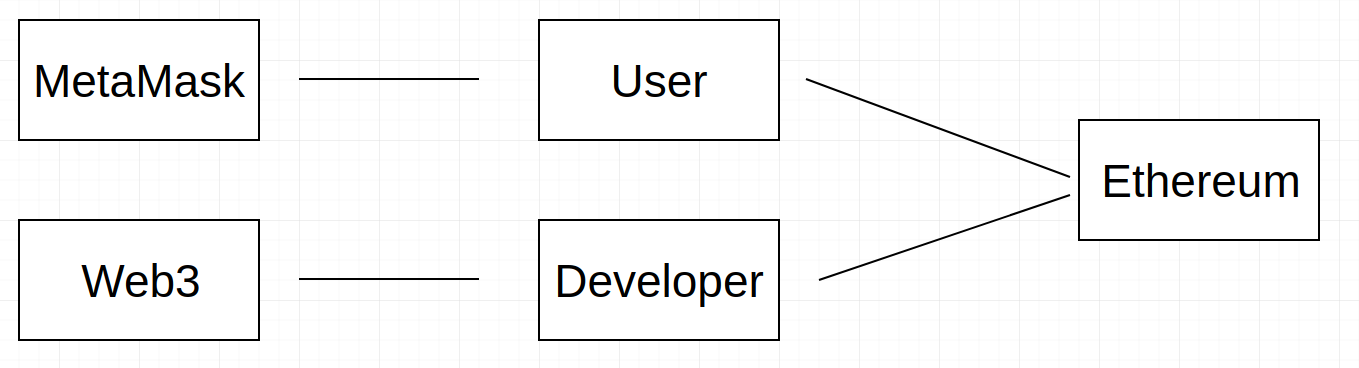
\includegraphics[width=0.9\textwidth]{metaweb3}
\caption[MetaWeb3]{Diagrama que representa el grupo de usuarios de cada herramienta}
\label{fig:metamask-web3}
\end{figure}

\subsubsubsection{Ganache CLI}

Siguiendo con el objetivo de testear nuestra aplicación y los contratos inteligentes, es el turno 
de Ganache. Ganache CLI (Command Line Interface) es parte de una suite de herramientas para el 
desarrollo de Ethereum llamada Truffle. Cabe destacar que pese a su gran adopción por parte de la 
comunidad, Truffle aún no se encuentra en una versión completamente estable por lo que es común
encontrarse con alguna de las herramientas con un comportamiento que no es el correcto.

Por su parte, Ganache nos proporciona una "blockchain personal" para deployar y testear contratos.
Es decir, nos brinda una blockchain local en tiempo de ejecución para que podamos probar allí
nuestros contratos.

Ganache utiliza Ethereumjs para simular un comportamiento de cliente completo y hacer más fácil,
sencillo y seguro el desarrollo de apps Ethereum.

Su instalación se da mediante el comando `npm install -g ganache-cli`
